\section{Příklad 1}

% Jako parametr zadejte skupinu (A-H)
\prvniZadani{H}
\centering
\subsection{Vypočítáme $R_{ekv}$ postupným zjednodušováním obvodu}
\begin{align*}
R_{45} &= \frac{R4 \times R5}{R4 + R5} = 201,4124 \Omega
\end{align*}

\begin{figure}[H]
    \centering
    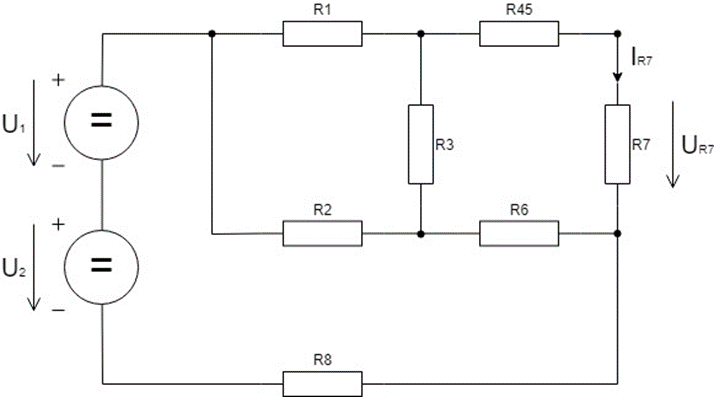
\includegraphics[width=0.6\textwidth]{fig/Pr1_1.png}
    \caption{$R_{45}~\sim~R_4,R_5$ paralelně}
    %\label{fig:mesh1}
\end{figure}

\begin{align*}
R_{457} = R_{45} + R_7 = 201,4124\Omega + 335\Omega = 536,4124\Omega
\end{align*}

\begin{figure}[H]
    \centering
    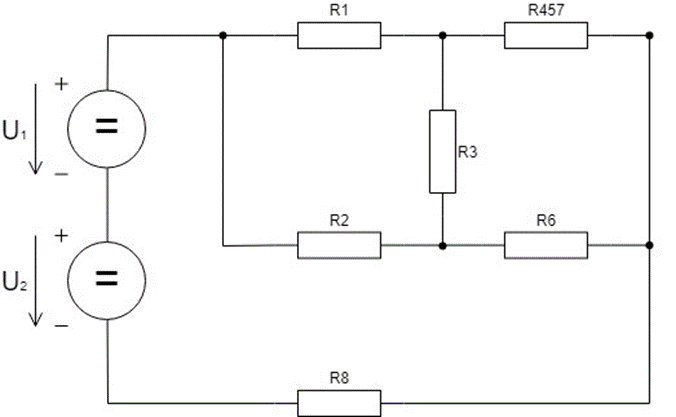
\includegraphics[width=0.6\textwidth]{fig/Pr1_2.png}
    \caption{$R_{457}~\sim~R_{45},R_7$ sériově}
    %\label{fig:mesh1}
\end{figure}

\begin{align*}
R_A &= \frac {R_1 \times R_2} {R_1 + R_2 + R_3} = \frac {408000\Omega} {1 540\Omega} = 264,9350\Omega\\
R_B &= \frac {R_1 \times R_3} {R_1 + R_2 + R_3} = \frac {176800\Omega} {1 540\Omega} = 114,8051\Omega\\
R_C &= \frac {R_2 \times R_3} {R_1 + R_2 + R_3} = \frac {156000\Omega} {1 540\Omega} = 101,2987\Omega
\end{align*}

\begin{figure}[H]
    \centering
    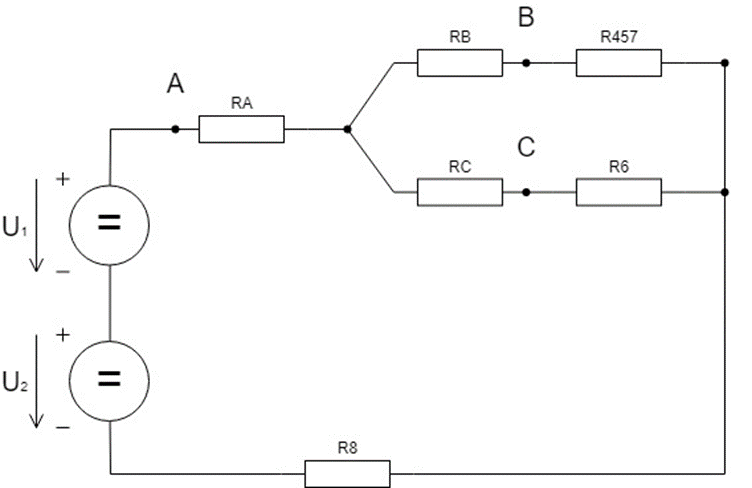
\includegraphics[width=0.6\textwidth]{fig/Pr1_3.png}
    \caption{Přechod trojúhelník $\rightarrow$ hvězda }
    %\label{fig:mesh1}
\end{figure}

\begin{align*}
R_{B457} &= R_B + R_{457} = 114,8051\Omega + 536,4124\Omega = 651,2175\Omega\\
R_{C6} &= R_C + R_6 = 101,2987\Omega + 870\Omega = 971,2987\Omega
\end{align*}

\begin{figure}[H]
    \centering
    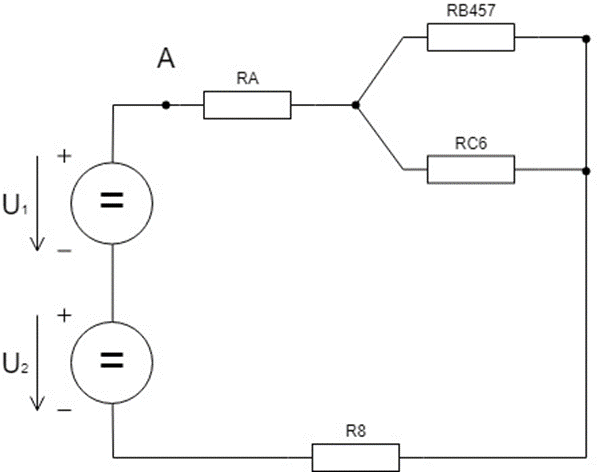
\includegraphics[width=0.6\textwidth]{fig/Pr1_4.png}
    \caption{$R_{B457}~\sim~R_B,R_{457}$ sériově,~$R_{C6}~\sim~R_C,R_6$ sériově}
    %\label{fig:mesh1}
\end{figure}

\begin{align*}
R_{B457C6} = \frac {R_{B457} \times R_{C6}} {R_{B457} + R_{C6}} = \frac {632 526,7111\Omega} {1 622,5162\Omega} = 389,8430\Omega
\end{align*}

\begin{figure}[H]
    \centering
    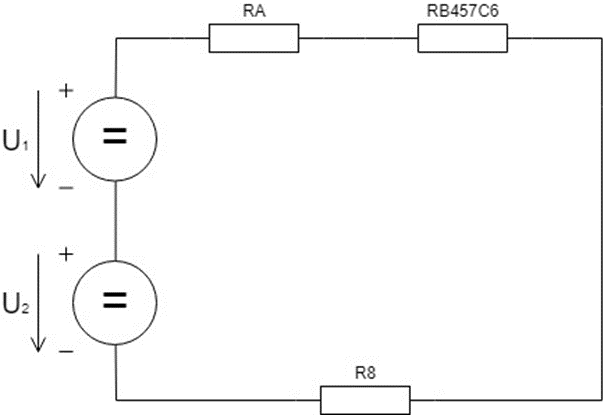
\includegraphics[width=0.6\textwidth]{fig/Pr1_5.png}
    \caption{$R_{B457C6}~\sim~R_{B457},R_{C6}$ paralelně}
    %\label{fig:mesh1}
\end{figure}

\begin{align*}
R_{AB457C6} &= R_A + R_{B457C6} = 264,9350\Omega + 389,8430\Omega = 654,778\Omega\\
R_{AB457C68} &= R_{AB457C6} + R_8 = 654,778\Omega + 265\Omega = 919,778\Omega\\
R_{ekv} &= R_{AB457C68} = 919,778\Omega
\end{align*}

\begin{figure}[H]
    \centering
    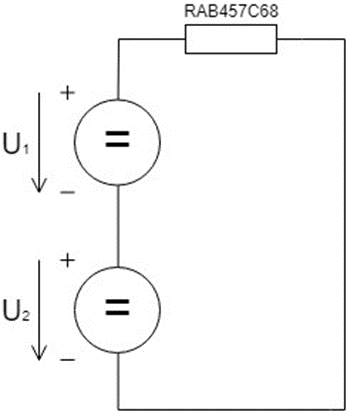
\includegraphics[width=0.3\textwidth]{fig/Pr1_6.png}
    \caption{$R_{AB457C6}~\sim~R_A,R_{B457C6}$ sériově, $R_{ekv}~\sim~R_{AB457C6},R_8$ sériově}
    %\label{fig:mesh1}
\end{figure}

\subsection{Zpětným chodem vypočítáme $U_{R7},~I_{R7}$ }

\begin{align*}
U &= U_1 + U_2 = 135V + 80V = 215 V\\
I &= \frac {U} {R_{ekv}} = \frac {215V} {919,778\Omega} = 0,2337 A\\ \\
U_{RAB457C6} &= R_{AB457C6} \times I = 654,778\Omega \times 0,2337 A = 153,0216 V\\
U_{R8} &= R_8 \times I = 265\Omega \times 0,2337 A = 61,9305 V\\ \\
U_{RA} &= R_A \times I = 264,9350\Omega \times 0,2337 A = 61,9153 V\\
U_{RB457C6} &= R_{B457C6} \times I = 389,8430\Omega \times 0,2337 A = 91,1063 V\\ \\
I_{RB457} &= \frac {U_{RB457C6}} {R_{B457}} = \frac {91,1063 V} {651,2175\Omega} = 0,1399 A\\
I_{RC6} &= \frac {U_{RB457C6}} {R_{C6}} = \frac {91,1063 V} {971,2987\Omega} = 0,0937 A
\end{align*}
\begin{align*}
U_{RB} &= R_B \times I_{RB457} = 114,8051\Omega \times 0,1399 A = 16,0612 V\\
U_{R457} &= R_{457} \times I_{RB457} = 536,4124\Omega \times 0,1399 A = 75,0440 V\\
U_{RC} &= R_C \times I_{RC6} = 101,2987\Omega \times 0,0937 A = 9,4916 V\\
U_{R6} &= R_6 \times I_{RC6} = 870\Omega \times 0,0937 A = 81,519 V
\end{align*}
\begin{figure}[H]
    \centering
    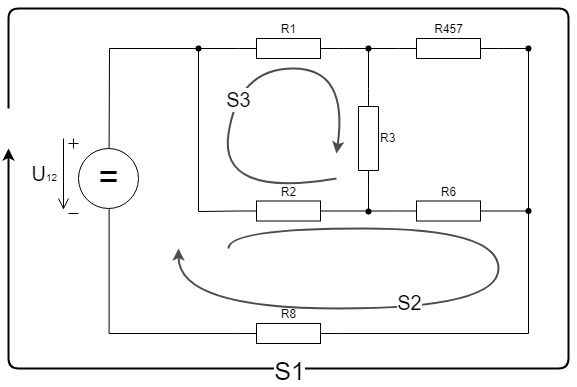
\includegraphics[width=0.6\textwidth]{fig/Pr1_7.jpg}
    \caption{Smyčka S1, S2, S3}
    %\label{fig:mesh1}
\end{figure}
\begin{align*}
S1: U_{R1} &+ U_{R457} + U_{R8} - U = 0 \textit{ (II Kir. Z)}\\
S2: U_{R2} &+ U_{R6} + U_{R8} - U = 0 \textit{ (II Kir. Z)}\\
S3: U_{R2} &- U_{R1} - U_{R3} = 0 \textit{ (II Kir. Z)}
\end{align*}
\begin{align*}
U_{R1} &= U - U_{R457} - U_{R8} = 215 V - 75,0440 V - 61,9305 V = 78,0255 V\\
U_{R2} &= U - U_{R6} - U_{R8} = 215 V - 81,519 V - 61,9305 V = 71,5505 V\\
U_{R3} &= U_{R1} - U_{R2} = 78,0255 V - 71,5505 V = 6,4750 V\\ \\
I_{R457} &= \frac {U_{R457}} {R_{457}} = \frac {75,0440 V} {536,4124\Omega} = 0,1398 A\\
I_{R457} &= \frac {U_{R45}} {R_{45}} = \frac {U_{R7}} {R_7}\\
U_{R45} &= I_{R457} \times R_{45} = 0,1398 A \times 201,4124\Omega = 28,1574 V\\ \\
\boldsymbol{U_{R7} }&=\boldsymbol{ I_{R457} \times R_7 = 0,1398 A \times 335\Omega = 46,8330 V}\\
\boldsymbol{I_{R7} }&=\boldsymbol{ I_{R457} = 0,1398 A}
\end{align*}